\documentclass[conference]{IEEEtran}

\usepackage{amssymb}
\usepackage{amsmath}
\usepackage{graphicx}
\usepackage{dcolumn}

\usepackage[T1]{fontenc}
\usepackage[utf8]{inputenc}
\usepackage[table]{xcolor}

\usepackage{booktabs}
\usepackage{multirow}
\usepackage{parcolumns}

\usepackage{todonotes}

\usepackage{hyperref}
\usepackage{float}
\usepackage{parcolumns}

\definecolor{pblue}{rgb}{0.13,0.13,1}
\definecolor{pgreen}{rgb}{0,0.5,0}
\definecolor{pred}{rgb}{0.9,0,0}
\definecolor{pgrey}{rgb}{0.46,0.45,0.48}

\usepackage{listings}
\lstset{language=Java,
  showspaces=false,
  showtabs=false,
  breaklines=true,
  showstringspaces=false,
  breakatwhitespace=true,
  commentstyle=\color{pgreen},
  keywordstyle=\color{pblue},
  numbers = left,
  stringstyle=\color{pred},
  basicstyle=\ttfamily,
%  moredelim=[il][\textcolor{pgrey}]{$$}
  moredelim=[is][\textcolor{pgrey}]{\%\%}{\%\%}
}

\def\checkmark{\tikz\fill[scale=0.4](0,.35) -- (.25,0) -- (1,.7) -- (.25,.15) -- cycle;}

\definecolor{lightyellow}{HTML}{fffdcc}
\definecolor{doublelightyellow}{HTML}{fffa9c}
\definecolor{lightgreen}{HTML}{dcffd4}
\definecolor{lightblue}{HTML}{e0ffff}
\definecolor{lightred}{HTML}{ffe0e0}
\definecolor{lightpink}{HTML}{ffe0ff}
\definecolor{lightorange}{HTML}{ffede0}
\definecolor{lightpurple}{HTML}{f0e0ff}
\newcommand{\highlightYellow}{\makebox[0pt][l]{\color{lightyellow}\rule[-4pt]{1\linewidth}{14pt}}}
\newcommand{\highlightGreen}{\makebox[0pt][l]{\color{lightgreen}\rule[-4pt]{1\linewidth}{14pt}}}
\newcommand{\highlightBlue}{\makebox[0pt][l]{\color{lightblue}\rule[-4pt]{1\linewidth}{14pt}}}
\newcommand{\highlightRed}{\makebox[0pt][l]{\color{lightred}\rule[-4pt]{1\linewidth}{14pt}}}
\newcommand{\highlightPink}{\makebox[0pt][l]{\color{lightpink}\rule[-4pt]{1\linewidth}{14pt}}}
\newcommand{\highlightOrange}{\makebox[0pt][l]{\color{lightorange}\rule[-4pt]{1\linewidth}{14pt}}}
\newcommand{\highlightPurple}{\makebox[0pt][l]{\color{lightpurple}\rule[-4pt]{1\linewidth}{14pt}}}
\newcommand{\highlightDarkyellow}{\makebox[0pt][l]{\color{doublelightyellow}\rule[-4pt]{1\linewidth}{14pt}}}

\lstnewenvironment{javacode}[1][]{\lstset{language=Java,escapechar=|,tabsize=2, breaklines=true, xleftmargin=.25in, keywordstyle=\color{pblue},basicstyle=\small,#1}}{}

\begin{document}

\title{Statement-level AST-based Clone Detection in Java using Resolved Symbols}
\author{\IEEEauthorblockN{1\textsuperscript{st} Simon Baars}
\IEEEauthorblockA{\textit{University of Amsterdam}\\
Amsterdam, the Netherlands \\
simon.mailadres@gmail.com}
}
%\affiliation{University of Amsterdam}

\maketitle

\thispagestyle{plain}
\pagestyle{plain}

\begin{abstract}
Duplication in source code is often seen as one of the most harmful types of technical debt as it increases the size of the codebase and creates implicit dependencies between fragments of code. Detecting such problems can provide valuable insight into the quality of systems and help to improve the source code. To correctly identify cloned code, contextual information should be considered, such as the type of variables and called methods.

Comparing code fragments including their contextual information introduces an optimization problem, as this information may be hard to retrieve. It can be ambiguous where contextual information resides and tracking it down may require to follow cross-file references. For large codebases, it could become time-consuming due to the sheer number of referenced symbols.

We propose a method to efficiently detect clones taking into account contextual information. We introduce a tool that uses an AST-parsing library named JavaParser to detect clones and retrieve contextual information. Our method parses the Abstract Syntax Tree retrieved from JavaParser into a graph structure, which is used to find clones. This graph maps the following relations for each statement in the codebase: the next statement, the previous statement, and the previous cloned statement.

We find that, when taking into account contextual information in our clone detection, 11\% fewer clones are found. Manually inspecting a sample of the difference, we find that they are less relevant for refactoring.
\end{abstract}

\begin{IEEEkeywords}
clone detection, context, java, parsing, static code analysis
\end{IEEEkeywords}

\section{Introduction}
%Most clone detection tools can be configured using thresholds. These thresholds indicate the minimum number of lines, tokens and/or statements that must be spanned for duplicate fragments to be considered clones. Often, such thresholds are intuitively chosen~\cite{li2006cp, roy2009mutation} or based on a quartile distribution of empirical data~\cite{alves2010deriving}. Using the maintainability score we can find support for which thresholds should be chosen to increase the chance to find clones that improve maintainability when refactored.
Duplicate code fragments are often considered as bad design~\cite{fowler2018refactoring}. They increasing maintenance efforts or causing bugs in evolving software~\cite{heitlager2007practical}. Changing one occurrence of a duplicated fragment may require changes in other occurrences~\cite{ostberg2014automatically}. Furthermore, duplicated code was shown to account for up to 25\% of total system volume~\cite{bruntink2005use}, entailing more code to be maintained.

Several tools have been proposed to detect duplication issues \cite{roy2009comparison, svajlenko2014evaluating, sheneamer2016survey}. These tools can find matching fragments of code, however do not take into account contextual information of code. An example of such contextual information is the name of used variables: many different methods with the same name can exist in a codebase. This can obstruct refactoring opportunities.

We describe a method to detect clones while taking into account the contextual information and introduce a tool to detect clones taking into account such contextual information. We run the tool over a corpus of 2,267 Java projects. We find that taking into account contextual information results in 11\% less clones than found when not taking this information into account. Manually inspecting a sample the difference, we find that all clones with different contextual information in our sample are less relevant for refactoring.

\begin{figure*}
\begin{parcolumns}{2}
\colchunk[1]{
\begin{javacode}
package com.sb.game;

import java.util.List;

public class GameScene
{
|\highlightYellow|	public void addToList(List l) {
|\highlightYellow|		l.add(getClass().getName());
|\highlightYellow|	}

	public void addTen(int x) {
|\highlightYellow|		x = x + 10; // add number
|\highlightYellow|		Notifier.notifyChanged(x);
|\highlightYellow|		return x;
	}
}
\end{javacode}}
\colchunk[2]{
\begin{javacode}
package com.sb.fruitgame;

import java.awt.List;

public class LoseScene
{
|\highlightYellow|	public void addToList(List l) {
|\highlightYellow|		l.add(getClass().getName());
|\highlightYellow|	}

	public void concatTen(String x) {
|\highlightYellow|		x = x + 10; // concat string
|\highlightYellow|		Notifier.notifyChanged(x);
|\highlightYellow|		return x;
	}
}
\end{javacode}}
\end{parcolumns}
\caption{Example of a clone that, although textually equal, is contextually different.}
\label{fig:type1}
\end{figure*}

\section{Background}
We first explain relevant code clone terminology and definitions. Next, we describe the JavaParser tool, used to retrieve contextual information of source code.

\subsection{Code clones}
We use two concepts to argue about code clones~\cite{roy2007survey}:
\\ \textbf{Clone instance}: A single cloned fragment.
\\ \textbf{Clone class}: A set of similar clone instances.

%\subsection{Clone Types}
Duplication in code is found in many different forms. Most often duplicated code is the result of a programmer reusing previously written code \cite{haefliger2008code, baxter1998clone}. Sometimes this code is then adapted to fit the new context. To reason about these modifications, several clone types have been proposed%. These clone types are described in Roy et al
~\cite{roy2007survey}:\\
\textbf{Type I:} Identical code fragments except for variations in whitespace (may be also variations in layout), and comments.\\
\textbf{Type II:} Structurally/syntactically identical fragments except variations in identifiers, literals, types, layout, and comments.\\
\textbf{Type III:} Copied fragments with further modifications. Statements can be changed, added or removed next to variations in identifiers, literals, types, layout, and comments.
Many studies adopt these clone types, analyzing them further and writing detection techniques for them \cite{sajnani2016sourcerercc, kodhai2010detection, van2019novel}. In this study, we mainly focus expanding type 1 clone detection to take into account contextual information.

\subsection{JavaParser}
JavaParser~\cite{tomassetti2017javaparser} is a Java library which allows parsing Java source files to an abstract syntax tree (AST). Integrated into JavaParser is a library named SymbolSolver. This library allows for the resolution of symbols using JavaParser. For instance, we can use it to trace references (methods, variables, types, etc) to their declarations (these referenced identifiers are also called ``symbols''). Using this, we can find the required contextual information.

To be able to trace referenced identifiers, SymbolSolver requires access to not only the analyzed Java project but also all its dependencies. This requires us to include all dependencies with the project. Along with this, SymbolSolver solves symbols in the JRE System Library (the standard libraries coming with every installation of Java) using the active Java Virtual Machine (JVM). %This has a big impact on performance efficiency. This is visible in our results, as displayed in Section~\ref{sec:clonetypeexperiments}.

\section{Motivating example} \label{sec:type1}
Most clone detection tools~\cite{kamiya2002ccfinder, semura2017ccfindersw, roy2008nicad, svajlenko2016bigcloneeval, svajlenko2014evaluating} detect type 1 clones by textually comparing code fragments (except for whitespace and comments). Although textually equal, method, type and variable references can still refer to different declarations. In such cases, refactoring opportunities could be invalidated. This can make the detected clones less suitable for refactoring purposes, as they require additional judgment regarding the refactorability of such a clone.

Figure~\ref{fig:type1} shows two clone classes. Merging these clone classes is very hard (and likely not desirable), as both cloned fragments describe different functional behavior. The first cloned fragment is a method that adds something to a \texttt{List}. However, the \texttt{List} objects to which something is added are different. Looking at the \texttt{import} statement above the class, one fragment uses the \texttt{java.util.List} and the other uses the \texttt{java.awt.List}. Both happen to have an \texttt{add} method, however their implementation is completely different.

The second cloned fragment shows how equally named variables can have different types and thus perform different functional concepts. The cloned fragment on the left adds a specific amount to an integer. The cloned fragment on the right concatenates a number to a String.

This shows that not all textually equal clones can be easily refactored.

\section{Contextual information}
To solve the issues identified in Section~\ref{sec:type1}, we expand clone detection by taking into account contextual information: cloned fragments have to be both textually \textit{and} contextually equal. We check contextual equality of two fragments by validating the equality of the fully qualified identifier (FQI) for referenced types, methods and variables. If an identifier is fully qualified, it means we specify the full location of its declaration (e.g. \texttt{com.sb.fruit.Apple} for an \texttt{Apple} object).

\subsection{Referenced Types}
Many object-oriented programming languages (like Java, Python, and C\#) require the programmer to import a type (or the class in which it is declared) before it can be used. Based on what is imported, the meaning of the name of a type can differ. For instance, if we import \texttt{java.util.List}, we get the interface which is implemented by all list data structures in Java. However, importing \texttt{java.awt.List}, we get a listbox GUI component for the Java Abstract Window Toolkit (AWT). These are entirely different functional concepts. To be sure we compare between equal types, we compare the FQI for all referenced types.

\subsubsection{Called methods}
A codebase can have several methods with the same name. The implementation of these methods might differ. When two code fragments call methods with an identical name or signature, they can still call different methods. Because of this, textually identical code fragments can differ functionally.

We compare the fully qualified method signature for all method references. A fully qualified method signature consists of the fully qualified name of the method, the fully qualified type of the method plus the fully qualified type of each of its arguments. For instance, an \texttt{eat} method could become
%\footnotesize{
\texttt{com.sb.Apple.eat(com.sb.Tool)}.
%}.

\begin{figure*}
  \centering
  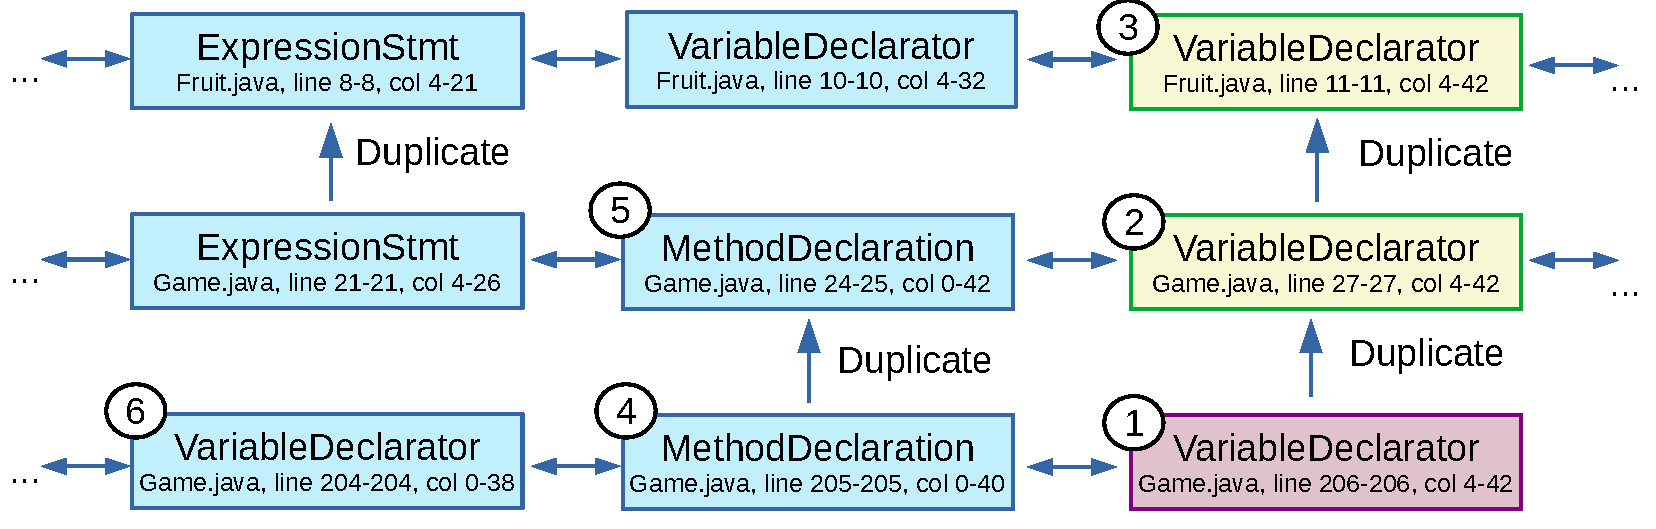
\includegraphics[width=1\textwidth]{img/CodeGraphExample}
  \caption{Example of a clone graph built by CloneRefactor.}
  \label{fig:clonegraph2}
\end{figure*}

\subsubsection{Variables}
In typed programming languages, each variable declaration should declare a name and a type. When we reference a variable, we only use its name. If we use variables with the same name but different types in different code fragments, the code can be functionally unequal but still textually equal.

The body of both methods in Figure~\ref{fig:type1} is equal. However, their functionality is not. The first method adds two numbers together and the other concatenates an integer and a String. Because of this, we compare cloned variable references by both their name and the FQI of their type.

\section{Clone Detection}\label{sec:clonedetection}
We develop a tool named CloneRefactor\footnote{CloneRefactor is available on GitHub: \url{https://github.com/SimonBaars/CloneRefactor}} that detects clones that can (relatively) easily be refactored. This tool uses JavaParser~\cite{tomassetti2017javaparser} to build an AST and to find contextual information (e.g. resolve symbols). We then propose a novel clone detection technique to detect clones using JavaParser.

%To detect clones, CloneRefactor parses the AST acquired from JavaParser to a graph structure. Based on this graph structure, clones are detected. Dependent on the type of clones being detected, transformations may be applied.

CloneRefactor uses JavaParser to read a project from disk and build an AST. %, one class file at a time.
Each AST is then converted to a directed graph that maps relations between statements. Based on this graph, CloneRefactor detects clone classes and verifies them using the configured thresholds. This process is explained in further detail over the following sections.
%\begin{itemize}
%  \item Amount of tokens.
%  \item Amount of statements.
%  \item Amount of lines.
%\end{itemize}


\subsection{Generating the clone graph}\label{sec:clonegraph}
CloneRefactor parses the AST obtained from JavaParser into a directed graph structure. We have chosen to base our clone detection around statements as the smallest unit of comparison. This means that a single statement cloned with another single statement is the smallest clone we can find. The rationale for this lies in both simplicity and performance efficiency. This means we won't be able to find when a single expression matches another expression, or even a single token matching another token. This is in most cases not a problem, as expressions are often small and do not span the minimal size to be considered a clone in the first place.

\begin{figure*}
  \centering
  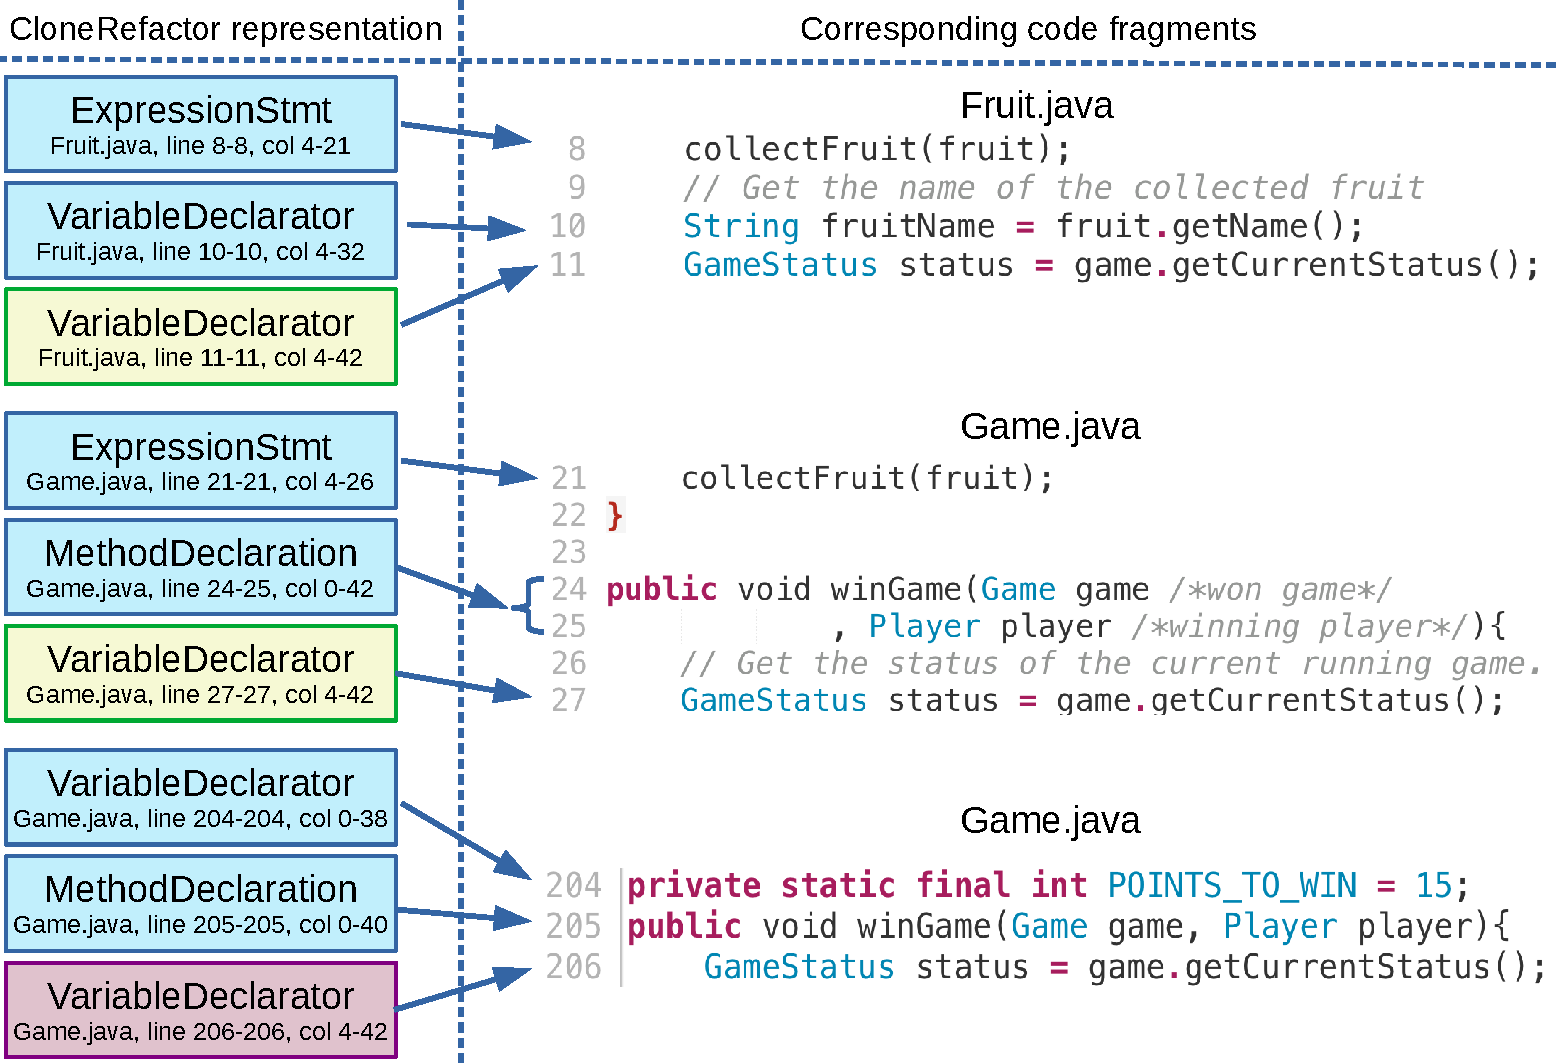
\includegraphics[width=1\textwidth]{img/CloneGraphCode}
  \caption{CloneRefactor extracts statements and declarations from source code.}
  \label{fig:clonegraph}
\end{figure*}

\subsection{Filtering the AST}
As a first step towards building the clone graph, we preprocess the AST to decide which AST nodes should become part of the clone graph: we exclude package declarations and import statements. These are omitted by most clone detection tools, as package declarations and import statements are most often generated by the IDE and not relevant for refactoring purposes.

\subsection{Building the clone graph}\label{sec:buildingclonegraph}
Building the clone graph consists of walking the AST in-order for each declaration and statement. For each declaration/statement found, we map the following relations:
\begin{itemize}
  \item The declaration/statement preceding it.
  \item The declaration/statement following it.
  \item The last \textbf{preceding} declaration/statement with which it is cloned.
\end{itemize}
We do not create a separate graph for each class file, so the statement/declaration preceding or following could be in a different file. While mapping these relations, we maintain a hashed map containing the last occurrence of each unique statement. This map is used to efficiently find out whether a statement is cloned with another. An example of such a graph is displayed in Figure~\ref{fig:clonegraph2}.

% \begin{figure*}
%   \centering
%   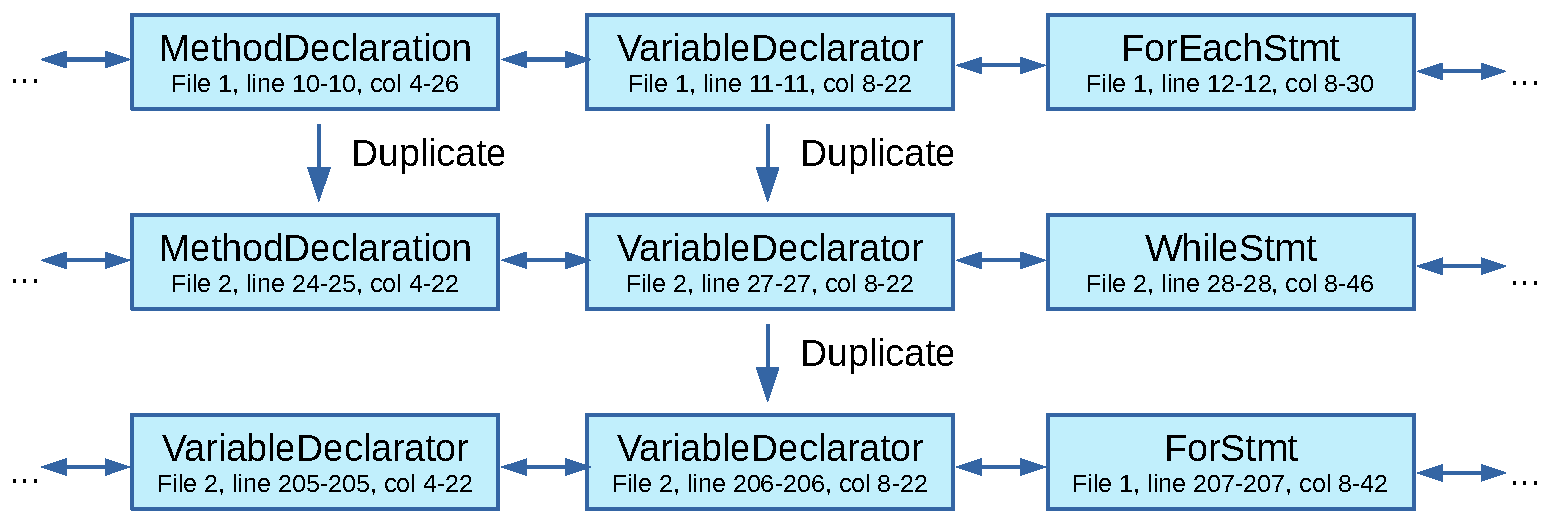
\includegraphics[width=1\textwidth]{img/CodeGraph2}
%   \caption{Abstract example of a part of a possible clone graph as built by CloneRefactor.}
%   \label{fig:clonegraphsimple}
% \end{figure*}

The relations \textit{next} and \textit{previous} in this graph are represented as a bidirectional arrow. The relations representing duplication are directed. %This is a restriction we've chosen as it creates an important constraint for the clone detection process. This process is explained in Section~\ref{sec:detectingclones}.

\subsection{Comparing Statements/Declarations} \label{sec:comparingstuff}
In the previous section, we described a ``duplicate'' relation between nodes in the clone graph built by CloneRefactor. Whether this duplicate relation exists between two nodes is determined by taking into account the contextual information. For \textit{method calls} we determine their fully qualified method signature for comparison with other nodes. For all \textit{referenced types} we use their fully qualified identifier (FQI) for comparison with other nodes. For \textit{variables} we compare their fully qualified type in addition to their name.

\subsection{Mapping graph nodes to code}
The clone graph, as explained in Section~\ref{sec:buildingclonegraph}, contains all declarations and statements of a software project. However, declarations and statements may themselves have child declarations and statements. To avoid redundant duplication checks, we exclude the body of each node.

Figure~\ref{fig:clonegraph} shows an example of how source code maps to AST nodes. On line 24-25 of the code fragment is a \texttt{MethodDeclaration}. The node corresponding with this MethodDeclaration denotes all tokens found on these two lines, line 24 and 25. Although the statements following this method declaration (those that are part of its body) officially belong to the method declaration, they are not included in its graph node. Because of that, in this example, the \texttt{MethodDeclaration} on line 24-25 will be considered a clone of the \texttt{MethodDeclaration} on line 205 even though their bodies might differ. Even the range (the line and column that this node spans) does not include its child statements and declarations.

\subsection{Detecting Clones} \label{sec:detectingclones}
After building the clone graph, we use it to detect clone classes. We start our clone detection process at the final location encountered while building the graph. As an example, we convert the code example shown in Figure~\ref{fig:clonegraph} to a clone graph as displayed in Figure~\ref{fig:clonegraph2}.

Using the example shown in Figure~\ref{fig:clonegraph2} and~\ref{fig:clonegraph} we can explain how we detect clones on the basis of this graph. Suppose we are finding clones for two files and the final node of the second file is a variable declarator. This node is represented in the example figure by the purple box (1). We then follow all ``duplicate'' relations until we have found all clones of this node (2 and 3). We now have a clone class of three clone instances each with a single node (1, 2 and 3).

Next, we move to the \textit{previous} line (4). Here again, we collect all duplicates of this node (4 and 5). For each of these duplicates, we check whether the node following it is already in the clone class we collected in the previous iteration. In this case, (2) follows (5) and (1) follows (4). This means that node (3) does not form a `chain' with other cloned statements. Because of this, the clone class of (1, 2 and 3) comes to an end. It will be checked against the thresholds, and if adhering to the thresholds, considered a clone.

We then go further to the previous node (6). In this case, this node does not have any clones. This means we check the (2 and 5, 1 and 4) clone class against the thresholds, and, if it adheres, consider it a clone. Dependent on the thresholds, this example can result in a total of two clone classes.

Eventually, following only the ``previous node'' relations, we can get from (6) to (2). When we are at that point, we will find only one cloned node for (2), namely (3). However, after we check this clone against the thresholds, we check whether it is a subset of any existing clone. If this is the case (which it is for this example), we discard the clone.

\section{Experiments and Results}
To compare the difference in detected clones when contextual information is considered, we compared the number of clones found when considering contextual information with when it is not considered. For this, we use a corpus of 2,267 Java projects including their dependencies \cite{baars2019towards}.

We find that 167,913 clones are found when contextual information is not considered, whereas 149,569 clones are found when it is considered. We manually analyse a sample of 50 clones that are not found when considering contextual information. We find that these clones are indeed hard to refactor because they describe different functional operations and can thus not be extracted to a new method. Also, most often they were not relevant because, based on our judgement, refactoring would not improve the code design. Often, different methods were called or variables of different types were used.

We also look into the difference in performance when taking into account contextual information. Detecting the clones in all 2,267 projects took 20.83 minutes when considering contextual information. When contextual information was not considered, it took 1.58 minutes. This is mainly because contextual information may be hard to retrieve, because the location of the contextual information may not be explicit. To find contextual information it may also be required to follow cross-file references. %The location of contextual information may also be implicit, which may require to seek through several files.

\section{Conclusion}
We propose a method to detect clones taking into account contextual information of source code. Contextual information is important because different functional concepts may turn up as clones because they are textually identical.

We define three aspects of source code as the contextual information:  a) the type of variable references; b) the location of method references; and c) the location of type references. When these references have the same name but point to different locations, clones may not be easily refactorable. Our results show that most such clones are not relevant for refactoring. This accounts for about 11\% of clones. This comes however with a performance trade-off: detecting clones with contextual information took 13 times longer than when not taking contextual information into account (1.6min vs 20.8min).

\bibliographystyle{plain}
\bibliography{references}

\end{document}
